\documentclass[a4paper, 12pt]{NUSThesis}
\usepackage{tikz}
\usepackage{lipsum}
\title{NUS Thesis Template}
\author{SHEN Zhou}
\prevdegrees{B.S. Lanzhou University}
\degree{Doctor of Philosophy}
\field{Physics}
\degreeyear{2020}

\begin{document}
\maketitle
\makedeclaration
\frontmatter
\begin{acknowledgments}
\lipsum[1-5]
\end{acknowledgments}
\tableofcontents
\begin{abstract}
\lipsum[1-3]
\end{abstract}
\listoftables
\listoffigures
\mainmatter
\chapter{Introduction}
\section{Introduction}
\lipsum[1-4]
\begin{table}[htpb]
    \centering
    \caption[short table caption]{This is long table caption test for single-space constriant. But
    it seems that I need to put more words here.}
    \begin{tabular}{ccc}
        \hline
        a & b & c\\
        \hline
    \end{tabular}
\end{table}
\lipsum[1-4]
\begin{figure}
    \centering
    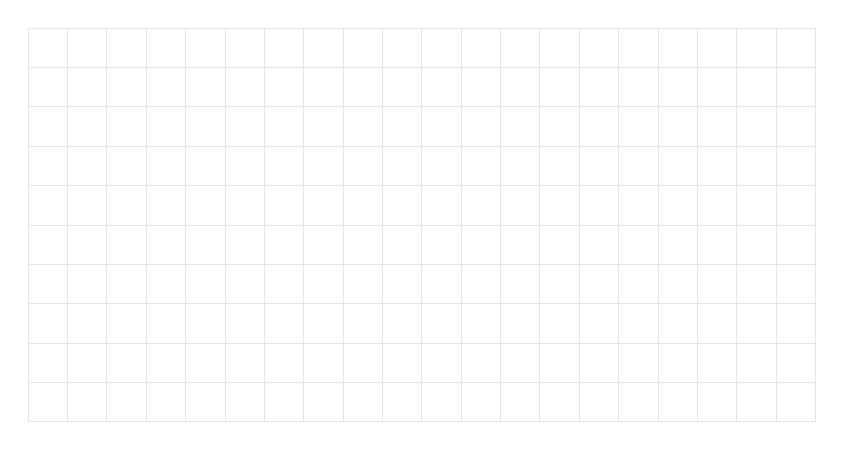
\begin{tikzpicture}
        \draw[help lines,step=5mm,gray!20] (0,0) grid (10,5);
    \end{tikzpicture}
    \caption[short figure caption]{This is long figure caption test for single-space constriant. But
    it seems that I need to put more words here.}
\end{figure}
\end{document}
